
En base a los anteriores requisitos el grupo de desarrollo ha generado diagramas para el software de \ac{S1} y \ac{S2}. A continuación se procederá a detallar cada uno de los distintos diagramas de cada uno de los sistemas . 

\section{Diagramas \textit{software} de S1}

\begin{figure}[H]
    \centering
    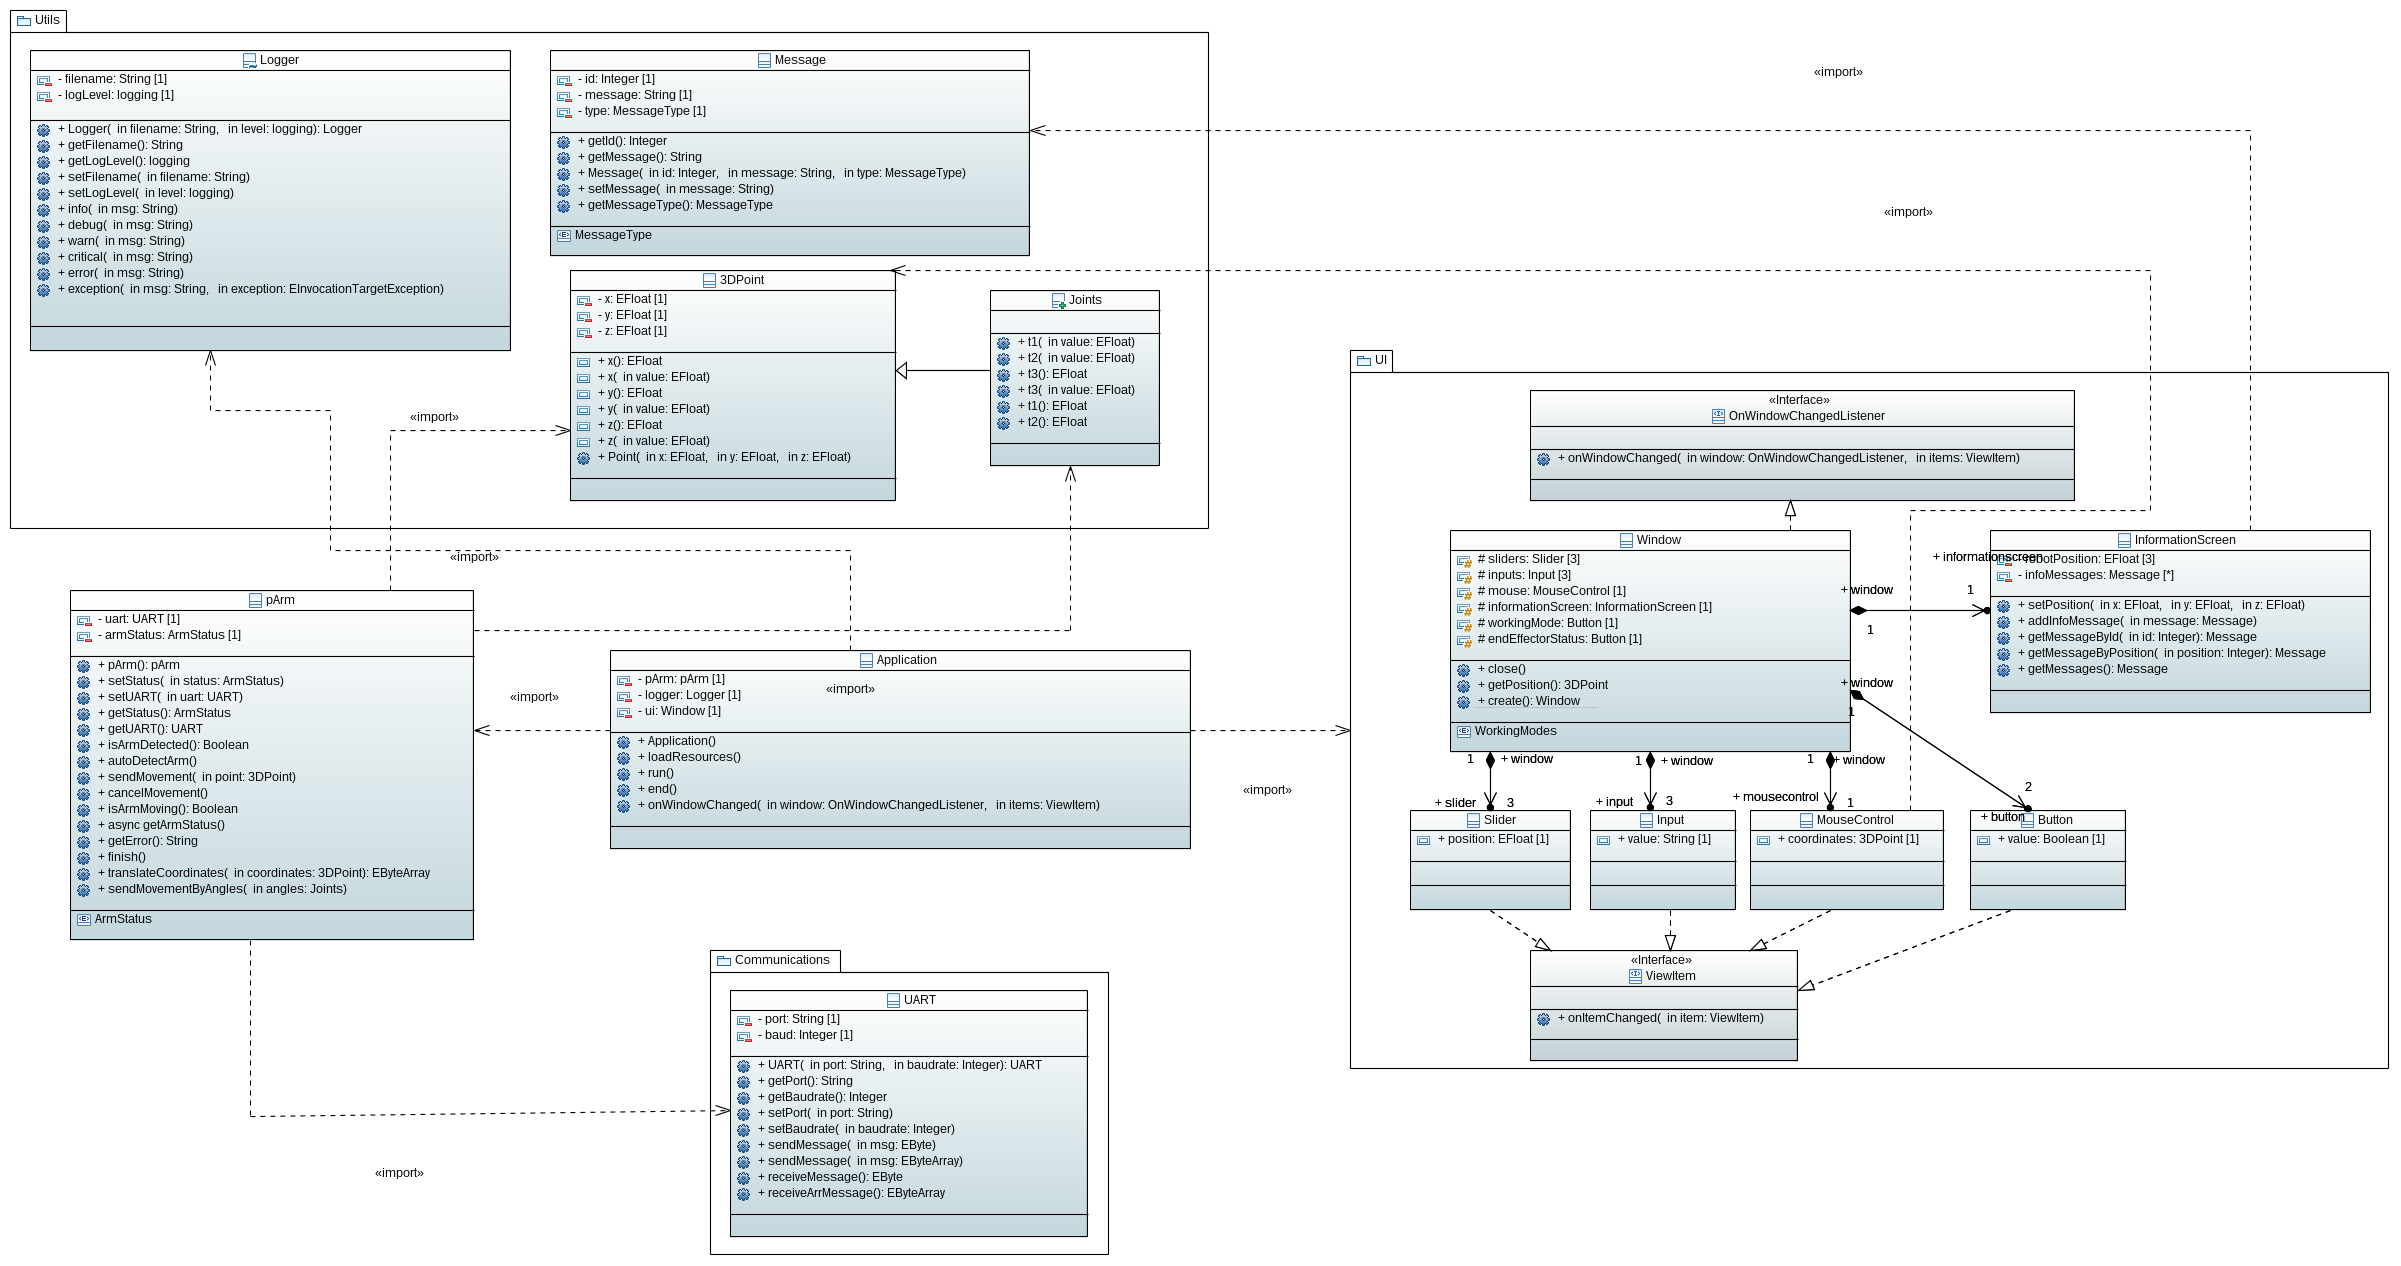
\includegraphics[width=\linewidth]{pictures/S1ClassDiagram.PNG}
    \caption{Diagrama de clases de \ac{S1}.}
    \label{fig:diagrama_clases_s1}
\end{figure}

En el diagrama \ref{fig:diagrama_clases_s1} se observa el diagrama de clases completo de \ac{S1}. Debido a su envergadura se procede a dividirlo en dos partes, a saber, la relacionada con la lógica del sistema y la relacionada con la GUI.

Para explicar la lógica del sistema \ac{S1} se hará una división por paquetes y posteriormente se procederá a explicar cada una de las clases que componen el paquete.

\begin{figure}[H]
    \centering
    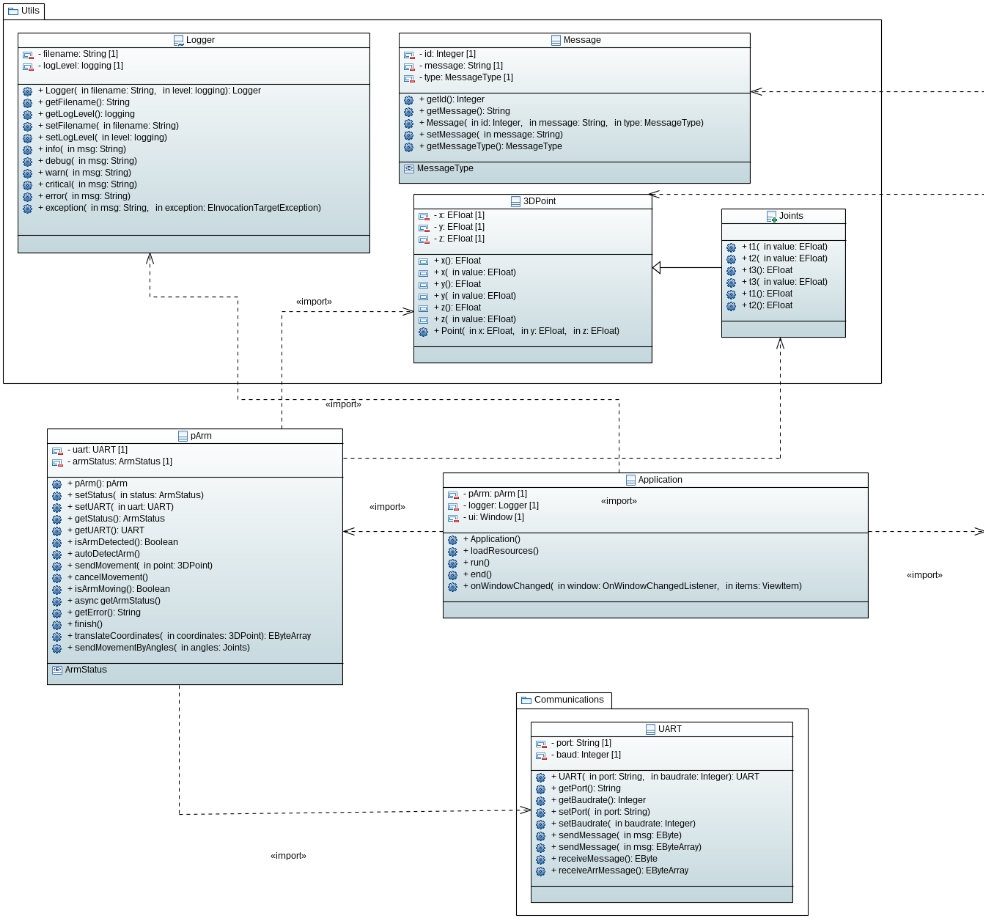
\includegraphics[width=\linewidth]{pictures/S1ClassDiagramLogic.PNG}
    \caption{Recorte del diagrama de clases de \ac{S1} el cual representa la lógica del sistema.}
    \label{fig:diagrama_clases_logica_s1}
\end{figure}

\begin{itemize}
    \item Paquete \texttt{Utils}: este paquete contiene clases cuyos objetos son instanciados con el objetivo de realizar labores genéricas que no están relacionadas de manera directa con la lógica o que no encajan en ningún otro paquete. Dentro de este paquete encontramos las siguientes clases:
    \begin{itemize}
        \item \texttt{Logger}: esta clase sirve para instanciar un objeto el cual genera archivos de registro del funcionamiento. Empleando ciertos métodos de esta clase, a lo largo del código, es posible guardar datos del sistema en un archivo, el cual es persistente en el tiempo. Posteriormente, se puede leer este archivo para poder hacer labores de \textit{debugging} tanto en las etapas de diseño como en la etapa de producción y despliegue.
        \item \texttt{Message}: los objetos de esta clase sirven para dar una estructura general a los diferentes mensajes que se mostrarán en la GUI con el objetivo de mostrar la información de manera uniforme.
        \item \texttt{3DPoint}: los objetos de esta clase representan puntos en el espacio cartesiano y se emplean para poder aunar las coordenadas en un solo objeto contenedor. Con esto se consigue simplificar la comunicación de los datos dentro del sistema. Los métodos que contiene son \textit{getters} y \textit{setters} de las distintas coordenadas.
        \item \texttt{Joints}: hereda de 3DPoints y los métodos son \textit{wrappers} de los \textit{getters} y lo \textit{setter} de esta.
    \end{itemize}
    \item Clase \texttt{pArm}: contiene los métodos necesarios para realizar los movimientos del brazo, inicializar las comunicaciones y posteriormente gestionarlas. Es la clase principal de la lógica del sistema.
    \item Clase \texttt{Application}: esta clase inicializa la aplicación y los recursos necesarios para el funcionamiento de esta. En ella se instancian objetos de las clases \texttt{pArm}, \texttt{Logger} y \texttt{ui}.
    \item Paquete \texttt{Communications}: contiene a la clase \texttt{UART}. Sirve para inicializar los puertos UART y la tasa de transmisión. Además, facilita los métodos para escribir en el canal de transmisión.
\end{itemize}

\begin{figure}[H]
    \centering
    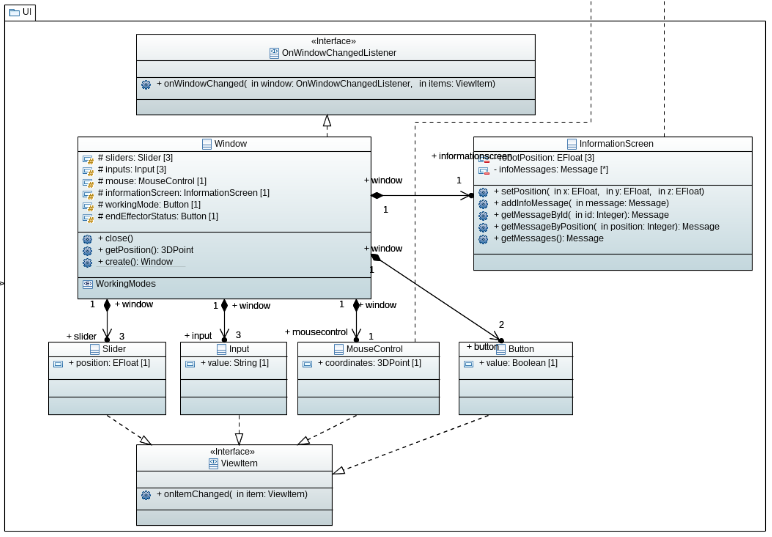
\includegraphics[width=\linewidth]{pictures/S1ClassDiagramGUI.PNG}
    \caption{Recorte del diagrama de clases de \ac{S1} el cual representa la interfaz gráfica de usuario.}
    \label{fig:diagrama_clases_GUI_s1}
\end{figure}

En este caso toda la GUI esta contenida dentro de un mismo paquete.

\begin{itemize}
    \item Clase \texttt{Window}: esta clase representa la ventana principal de la aplicación donde se encuentran todos los elementos con el que le usuario puede interactuar.
    \item Clase \texttt{Slider}: \textit{widget} de tipo \textit{Slider} que aparece dentro de la ventana principal y sirve para definir valores de las coordenadas cartesianas y angulares de manera gráfica.
    \item Clase \texttt{Input}: \textit{widget} de tipo \textit{SpinBox} que parece dentro de la ventana principal y sirve para definir valores de las coordenadas cartesianas y angulares de manera gráfica directamente con el valor en concreto.
    \item Clase \texttt{MouseControl}: clase empleada para obtener las coordenadas del ratón.
    \item Clase \texttt{Button}: \textit{widget} de tipo \textit{Button} que se emplea para desencadenar acciones en el sistema.
    \item Clase \texttt{InformationScreen}: panel que contiene texto, el cual informa al operario de distintos datos relacionados con el brazo y la aplicación
    \item Interfaz \texttt{ViewItem}: función de \textit{callback} para tener constancia de los cambios en los distintos \textit{widgets}.
    \item Interfaz \texttt{OnWindowChangeListener}: función de \textit{callback} para tener constancia de los cambios en la ventana de la interfaz.
\end{itemize}


\begin{figure}[H]
    \centering
    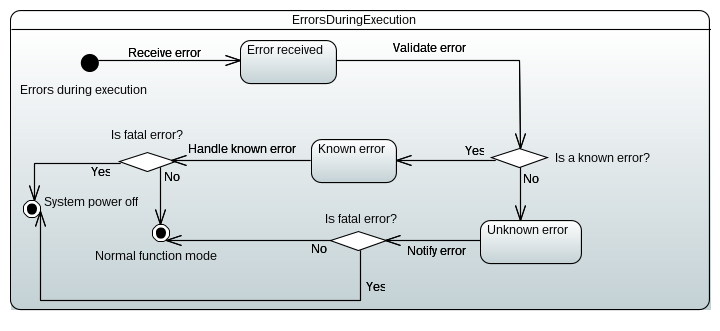
\includegraphics[width=\linewidth]{pictures/S1ErrorsDuringExecution.PNG}
    \caption{Diagrama de estados del tratamiento de errores de \ac{S1}.}
    \label{fig:diagrama_estados_error_s1}
\end{figure}

El diagrama \ref{fig:diagrama_estados_error_s1} representa el tratamiento de errores en el \ac{S1}.
Se observa que, dependiendo de si los errores son fatales o no, el sistema se apagará o seguirá funcionando.

\begin{figure}[H]
    \centering
    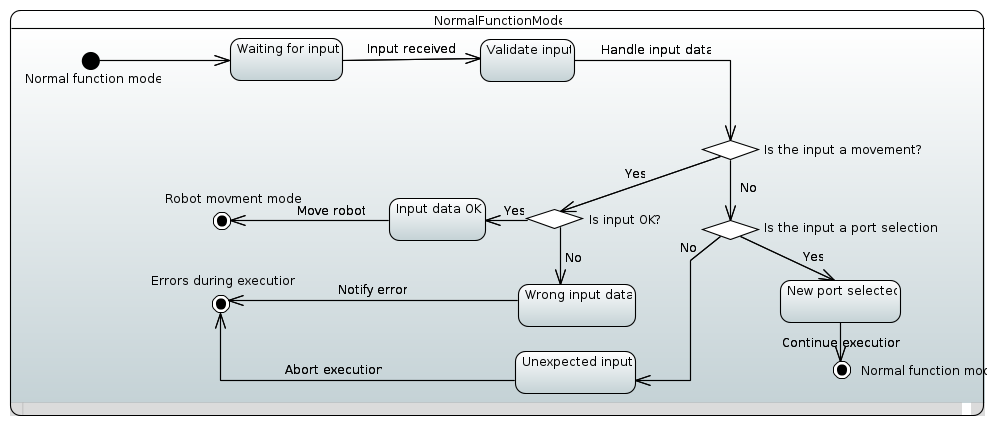
\includegraphics[width=\linewidth]{pictures/S1NormalFunctionMode.PNG}
    \caption{Diagrama de estados del funcionamiento normal de \ac{S1}.}
    \label{fig:diagrama_estados_normal_s1}
\end{figure}

En este diagrama se observa que, durante el funcionamiento normal de la aplicación, se puede interactuar con esta o bien seleccionando un puerto o bien definiendo un movimiento que el brazo habrá de realizar.
En el primer caso, la aplicación vuelve al funcionamiento normal de manera directa, mientras que en el segundo caso, si el movimiento es correcto se procede al modo de movimiento. Si por el contrario es un dato erróneo, se notifica del error.

\begin{figure}[H]
    \centering
    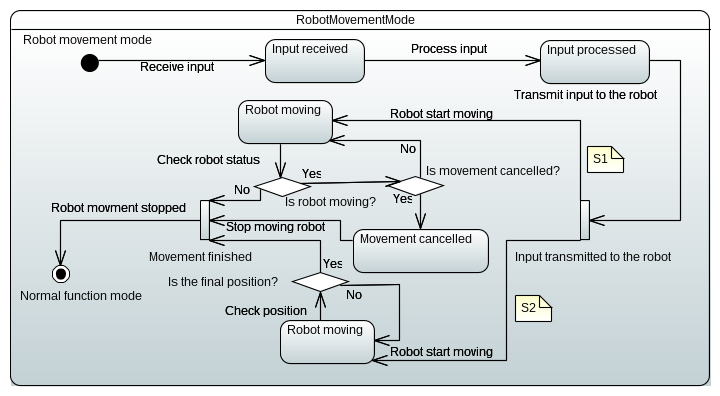
\includegraphics[width=\linewidth]{pictures/S1RobotMovementMode.PNG}
    \caption{Diagrama que representa el movimiento del brazo robótico tanto en \ac{S1} como en \ac{S2}.}
    \label{fig:diagrama_estados_movimiento_s1}
\end{figure}

Tras recibir una orden de movimiento esta es interpretada y los valores de la posición destino son transmitidos a \ac{S2}. En este momento, los dos sistemas empiezan a funcionar de manera concurrente.
\ac{S1} se encargará de monitorizar si se recibe una orden de cancelar movimiento por parte del usuario y esperara a que \ac{S2} termine el movimiento.
Por otro lado, \ac{S2} comprobará si su posición actual coincide con la posición destino y procederá a moverse en dirección a esta hasta que la alcance.

\begin{figure}[H]
    \centering
    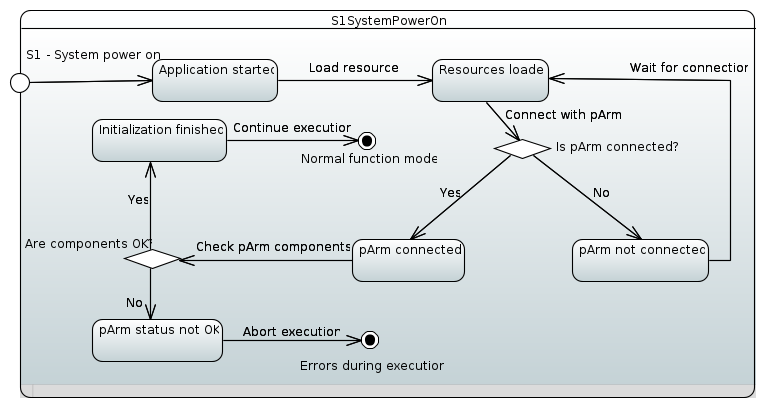
\includegraphics[width=\linewidth]{pictures/S1SystemPowerOn.PNG}
    \caption{Diagrama de estados del encendido de \ac{S1}.}
    \label{fig:diagrama_estados_encendido_s1}
\end{figure}

El sistema \ac{S1} inicia la aplicación y carga los recursos necesarios para que esta pueda empezar a mostrarse por pantalla. Al conectarse con el brazo, \ac{S1} comprueba que \ac{S2} esté en un estado correcto y de ser así finaliza la inicialización del sistema y permite la interacción con \ac{S2}.

\begin{figure}[H]
    \centering
    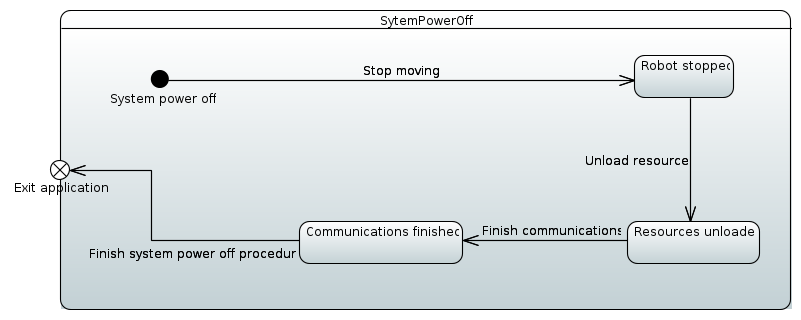
\includegraphics[width=\linewidth]{pictures/S1SystemPowerOff.PNG}
    \caption{Diagrama de estados del apagado de \ac{S1}.}
    \label{fig:diagrama_estados_apagado_s1}
\end{figure}

Para apagar el sistema, este tiene que asegurarse que \ac{S2} no está realizando un movimiento. En caso contrario, \ac{S1} ordena a \ac{S2} que lo cancele. Tras \ac{S1} asegurarse que el movimiento ha parado, se cierra.

\section{Diagramas \textit{software} de S2}

En el caso de los diagramas de \ac{S2} cabe destacar que los estados de error funcionan en cascada, es decir, dado que cada uno de los diagramas de estados representa una función del código, estas podrán tener errores en su ejecución y estos errores se irán propagando en cascada hacia niveles más altos de abstracción a lo largo de las diferentes funciones que han sido invocadas.

\begin{figure}[H]
    \centering
    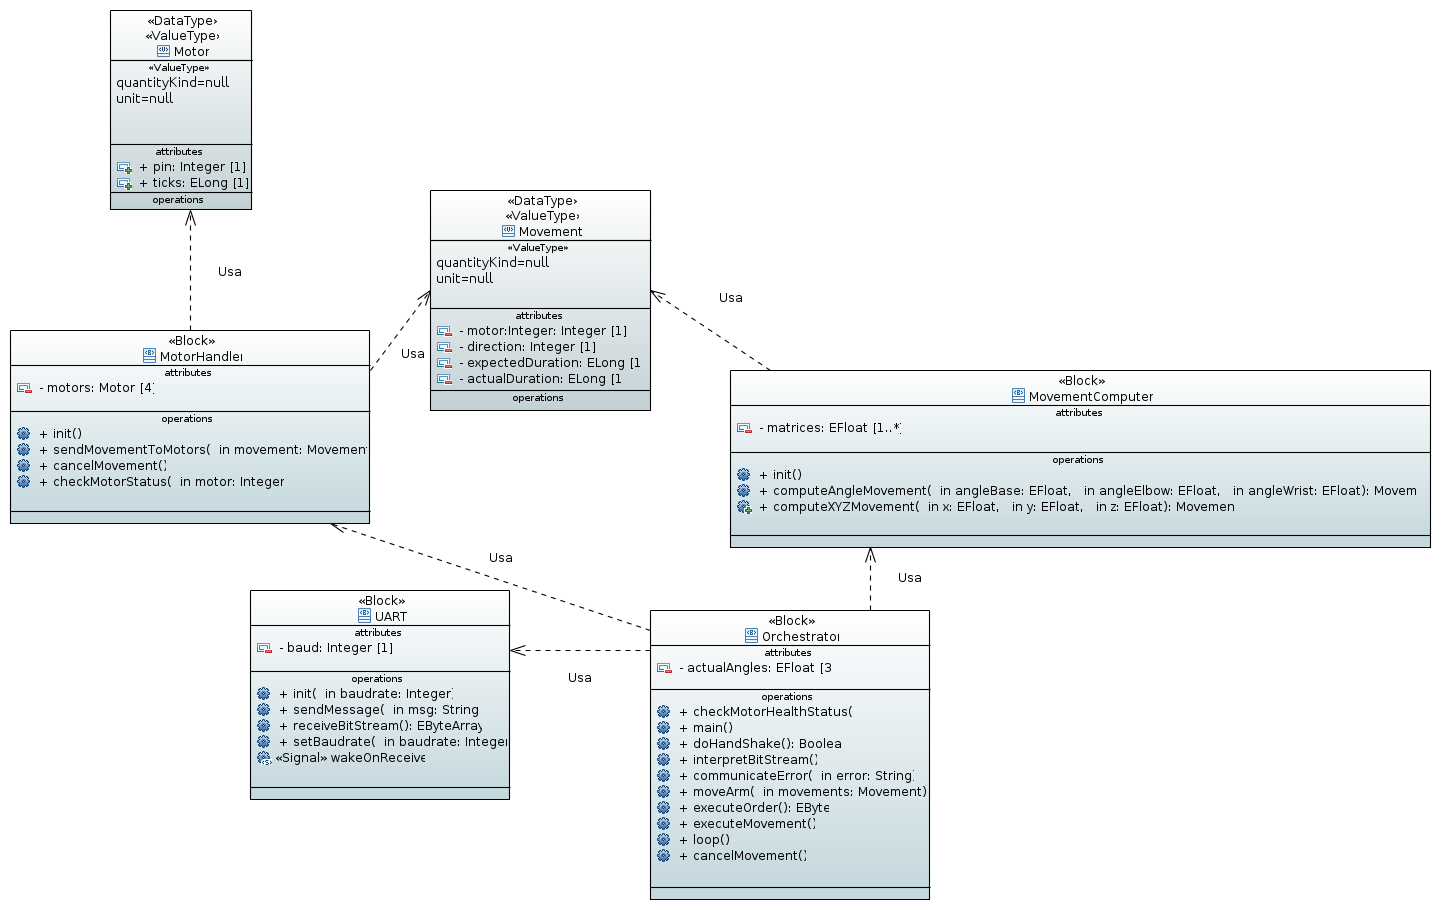
\includegraphics[width=\linewidth]{pictures/S2BlockDiagram.PNG}
    \caption{Diagrama de bloques de \ac{S2}.}
    \label{fig:diagrama_bloques_s2}
\end{figure}

En el diagrama \ref{fig:diagrama_bloques_s2} se pueden observar los bloques que componen \ac{S2} además de dos tipos de datos los cuales han sido creados para facilitar el control de los motores del brazo.

A continuación se explican cada uno de los bloques:

\begin{itemize}
    \item \texttt{MotorHandler}: este bloque es capaz de controlar los motores de manera directa empleando el tipo de dato ``\texttt{Movement}'' enviando la señal necesaria para realizar el movimiento requerido. Además, permite verificar el estado de los motores y cancelar los movimientos si esto fuese necesario.
    
    \item \texttt{UART}: este bloque es el encargado de la comunicación asíncrona entre \ac{S1} y \ac{S2}. Controla la tasa de baudios de la comunicación y realiza la transmisión y la recepción de información hasta y desde \ac{S1}. A través de este bloque se reciben las órdenes procedentes de \ac{S1} y se envían los errores y la posición del brazo a S1 desde \ac{S2}.
    
    \item \texttt{Orchestrator}: encargado de coordinar los demás bloques. En él se encuentra la lógica principal de \ac{S2}. Algunas de sus funciones más importantes son interpretar el flujo de bits que llega desde S1 para obtener una orden concreta; ordenar el movimiento del brazo empleando los demás bloques o hacer la sincronización inicial entre \ac{S1} y  \ac{S2}. Posteriormente se entrará en mayor detalle sobre el comportamiento de este bloque al analizar los diagramas de estados.
    
    \item \texttt{MovementComputer}: se encarga de computar el movimiento que se tendrá que comunicar a los motores. Para ello deberá obtener las posiciones deseadas gracias al bloque \texttt{UART} y al ``\texttt{Orchestrator}''.
\end{itemize}

A continuación se explican las dos estructuras de datos que se aprecian en el diagrama \ref{fig:diagrama_bloques_s2}

\begin{itemize}
    \item \texttt{Motor}: este tipo de dato es empleado por ``\texttt{MotorHandler}'' para saber a qué pin debe mandar la señal ``\ac{PWM}'' que gobierna los motores y durante cuántos \textit{ticks} deberá estar activa dicha señal
    
    \item \texttt{Movement}: ``\texttt{MovementComputer}'' genera un vector de 3 posiciones de este tipo de dato, uno por cada motor de giro del brazo. El atributo \texttt{motor} guarda un entero que representa uno de los motores del brazo; \texttt{direction} sirve para conocer la dirección de giro de dicho motor; \texttt{expectedDuration} guarda la duración.
\end{itemize}

A continuación se explican los diagramas de estados de cada uno de los métodos que aparecen en el diagrama de bloques general.

En el caso del \texttt{Orchestrator} tenemos los siguientes diagramas:

\begin{figure}[H]
    \centering
    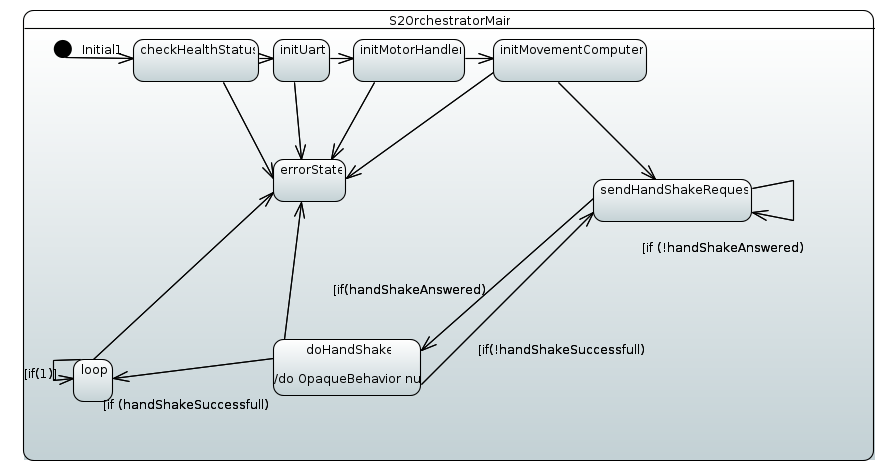
\includegraphics[width=1\linewidth]{pictures/S2OrchestratorMain.PNG}
    \caption{Diagrama de estados del método \texttt{main()} del \textit{orchestrator}.}
    \label{fig:fun_main_orchestrator}
\end{figure}

Este método solo se ejecutará una vez, en cuanto el sistema se ponga en marcha. 

\begin{enumerate}
    \item \texttt{checkHealthStatus}: se verifica la situación de los componentes del brazo robótico para confirmar que todos están en un estado adecuado para el funcionamiento. 
    \item \texttt{initUart}: se inicializa la \ac{UART} definiendo una tasa de baudios concreto.
    \item \texttt{initMotorHandler}: se inicializa el controlador de los motores.
    \item \texttt{initMovementComputer}: se inicializa el computador de movimientos.
    \item \texttt{sendHandShakeRequest} : se manda una petición de \textit{handshake} para verificar si hay algún ordenador conectado. Si se detecta alguno se pasa al siguiente estado. Si no, se mantiene en ese estado mandando peticiones.
    \item \texttt{doHandShake}: si en el estado anterior se detecta un ordenador se pasa a este estado. Se realiza una serie de intercambios de información para verificar que el ordenador conectado es adecuado para el control del brazo.
    \item \texttt{loop}: se pasa al bucle de funcionamiento si el \textit{handshake} ha sido correcto.
    \item \texttt{errorState}: estado de error al que se llega si en alguno de los estados ocurre algún problema inesperado. 
\end{enumerate}

\begin{figure}[H]
    \centering
    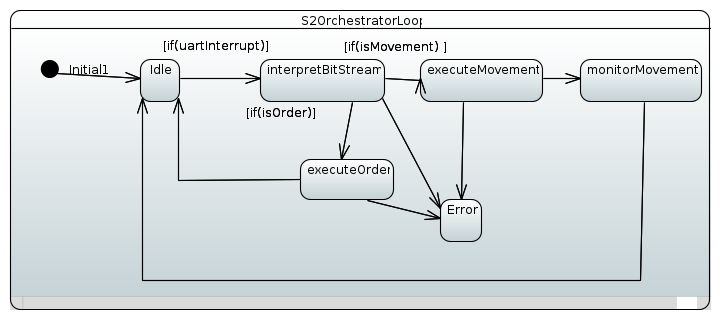
\includegraphics[width=1\linewidth]{pictures/S2OrchestratorLoop.PNG}
    \caption{Diagrama de estados del método \texttt{loop()} del \textit{orchestrator}.}
    \label{fig:fun_loop_orchestrator}
\end{figure}

Este método es el bucle principal del brazo robotico. Tras ejecutar \texttt{main()} el sistema entrará en este bucle y no saldrá hasta que se apaga.

\begin{enumerate}
    \item \texttt{Idle}: el brazo se encuentra ocioso y a la espera de una orden desde \ac{S1}.
    \item \texttt{interpretBitStream}: tras una interrupción de la \ac{UART}, \ac{S2} entiende que hay una orden o movimiento procedentes de \ac{S1} y se avanza a este estado. La trama de bits es interpretada para saber si es una orden o un movimiento.
    \item \texttt{executeMovement}: si tras interpretar la trama de bits resulta que es un movimiento, el sistema avanza a este estado y se ponen en marcha los demás bloques para poder generar un movimiento en los motores en base a la posición recibida desde \ac{S1}
    \item \texttt{executeOrder}: si tras interpretar la trama de bits resulta que es una orden, el sistema avanza a este estado y se ponen en marcha los bloques necesarios para ejecutar dicha orden.
    \item \texttt{monitorMovement} : tras empezar a ejecutar un movimiento, \ac{S2} empieza a monitorizarlo para poder determinar cuándo se ha terminado o, si es cancelado, actualizar la posición en la que se ha quedado el brazo.
    \item \texttt{errorState}: estado de error al que se llega si en alguno de los estados ocurre algún problema inesperado. 
\end{enumerate}

\begin{figure}[H]
    \centering
    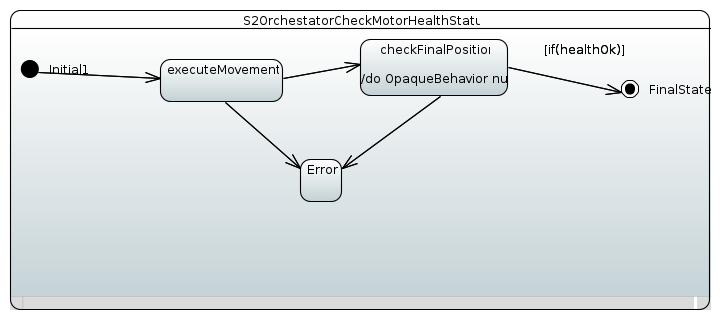
\includegraphics[width=1\linewidth]{pictures/S2OrchestratorCheckMotorHealthStatus.PNG}
    \caption{Diagrama de estados del método \texttt{CheckMotorHealthStatus()} del \textit{orchestrator}.}
    \label{fig:fun_check_motor_health_status_orchestrator}
\end{figure}

Este método comprueba el estado de los motores para asegurar que estos tienen un funcionamiento correcto antes de recibir cualquier orden de movimiento.

\begin{enumerate}
    \item \texttt{executeMovement}: se ejecuta un movimiento a una posición en la que todos los fines de carrera sean activados.
    \item \texttt{checkFinalPosition}: se verifica que todos los fines de carrera han sido alcanzados pudiendo concluir que el brazo es capaz de mover todos sus motores.
\end{enumerate}

\begin{figure}[H]
    \centering
    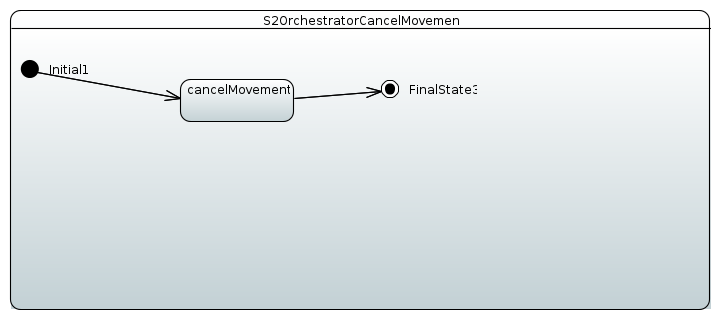
\includegraphics[width=1\linewidth]{pictures/S2OrchestratorCancelMovement.PNG}
    \caption{Diagrama de estados del método \texttt{CancelMovement()} del \textit{orchestrator}.}
    \label{fig:fun_cancel_movement_orchestrator}
\end{figure}

Este método finaliza un movimiento que se este realizando.

\begin{itemize}
    \item \texttt{cancelMovement}: se cancela el movimiento y se guarda la posición actual del brazo.
\end{itemize}

\begin{figure}[H]
    \centering
    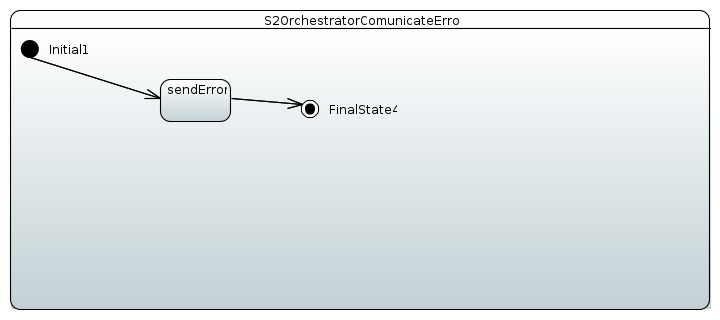
\includegraphics[width=1\linewidth]{pictures/S2OrchestratorComunicateError.PNG}
    \caption{Diagrama de estados del método \texttt{ComunicateError()} del \textit{orchestrator}.}
    \label{fig:fun_comunicate_error_orchestrator}
\end{figure}

Este método comunica un error a \ac{S1}.

\begin{itemize}
    \item \texttt{sendError}: se envía una trama de bits que representa un error ocurrido en \ac{S2}.
\end{itemize}

\begin{figure}[H]
    \centering
    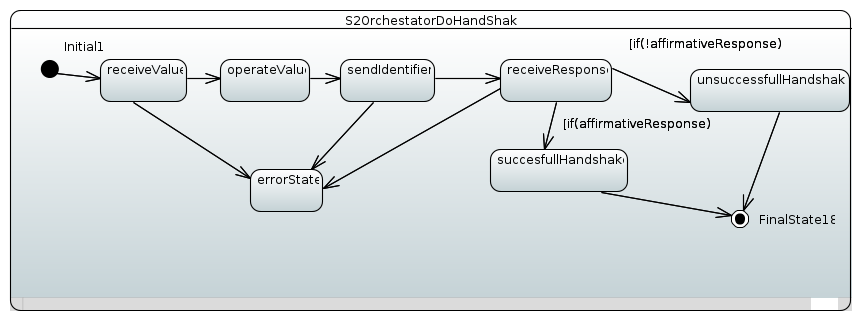
\includegraphics[width=1\linewidth]{pictures/S2OrchestratorDoHandShake.PNG}
    \caption{Diagrama de estados del método \texttt{DoHandShake()} del \textit{orchestrator}.}
    \label{fig:fun_do_hand_shake_orchestrator}
\end{figure}

Este método es el encargado de autenticar a los dispositivos entre sí y configurar un canal para su posterior comunicación

\begin{enumerate}
    \item \texttt{receiveValue}: se realizan los procedimientos necesarios para recibir un valor desde \ac{S1} a través de la \ac{UART}.
    \item \texttt{operateValue}: se realiza una operación matemática con el valor recibido para generar de esta manera un identificador.
    \item \texttt{sendIdentifier}: se envía dicho identificador de vuelta a \ac{S1}.
    \item \texttt{receiveResponse}: se recibe la respuesta de \ac{S1} para saber si el \textit{handshake} ha sido realizado con éxito.
    \item \texttt{successfulHandshake}: en caso de que en el estado
    \texttt{receiveResponse} se haya recibido una respuesta afirmativa se pasa a este estado que representa que los dispositivos han conseguido autenticarse entre sí.
    \item \texttt{unsuccessfulHandshake}: en caso de que en el estado \texttt{receiveResponse} se haya recibido una respuesta negativa se pasa a este estado que representa que los dispositivos no han conseguido autenticarse
    entre sí.
    \item \texttt{errorState}: estado de error al que se llega si en alguno de los estados ocurre algún problema inesperado. 
\end{enumerate}

\begin{figure}[H]
    \centering
    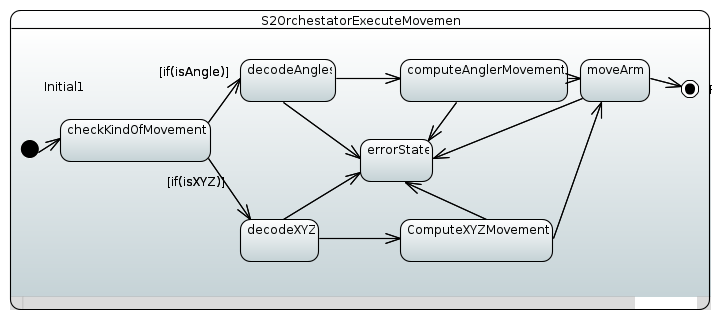
\includegraphics[width=1\linewidth]{pictures/S2OrchestratorExecuteMovement.PNG}
    \caption{Diagrama de estados del método \texttt{ExecuteMovement()} del \textit{orchestrator}.}
    \label{fig:fun_execute_movement_orchestrator}
\end{figure}

Este método es el encargado de, una vez recibida la trama de bits que representa un movimiento desde S1, decidir si el movimiento ha sido representado como ángulos o posiciones cartesianas y posteriormente ordenar las operaciones necesarias para que se generen las señales \ac{PWM} que moverán los motores.

\begin{enumerate}
    \item[1.] \texttt{checkKindOfMovement}: se verifica si el movimiento ha sido transmitido como una posición cartesiana o como unos ángulos destino para los motores y se procede en consecuencia.
    \item[2.] \texttt{decodeAngles}: en caso de que fueran ángulos, se transita a este estado. Se interpreta la trama de bits y se obtiene el valor numérico de los ángulos.
    \item[2.1.] \texttt{computeAngleMovement}: se realizan comprobaciones para verificar que los ángulos están dentro de los limites del brazo y se procede a generar el vector de movimientos que se necesitan hacer para conseguir llegar desde la posición actual a la posición destino.
    \item[3.] \texttt{decodeXYZ}: en caso de que fueran posiciones cartesianas se transita a este estado. Se interpreta la trama de bits y se obtienen las coordenadas en centímetros.
    \item[3.1.] \texttt{computeXYZMovements}: para simplificar los cálculos matemáticos posteriores las posiciones cartesianas se convierten en ángulos. Se verifica si los ángulos están dentro de los limites del brazo y se procede a generar el \textit{array} de movimientos que se necesitan hacer para conseguir llegar desde la posición actual a la posición destino.
    \item[4.] \texttt{moveArm}: se envían los movimientos a los motores.
    \item[5.] \texttt{errorState}: estado de error al que se llega si en alguno de los estados ocurre algún problema inesperado. 
\end{enumerate}

\begin{figure}[H]
    \centering
    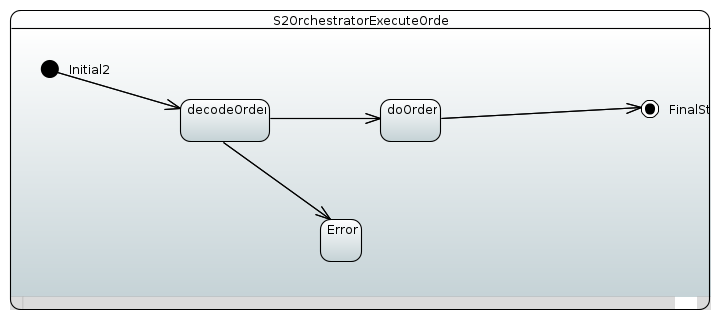
\includegraphics[width=1\linewidth]{pictures/S2OrchestratorExecuteOrder.PNG}
    \caption{Diagrama de estados del método \texttt{ExecuteOrder()} del \textit{orchestrator}.}
    \label{fig:fun_execute_order_orchestator}
\end{figure}

Este método es el encargado de, una vez recibida la trama de bits que representa una orden distinta de realizar un movimiento desde S1, decodificar dicha orden y realizarla.

\begin{enumerate}
    \item \texttt{decodeOrder}: se interpreta la trama de bits para obtener la orden proveniente desde S1.
    \item \texttt{doOrder}: se ejecuta la orden obtenida en el estado anterior.
    \item \texttt{Error}: estado de error al que se llega si en alguno de los estados ocurre algún problema inesperado. 
\end{enumerate}

\begin{figure}[H]
    \centering
    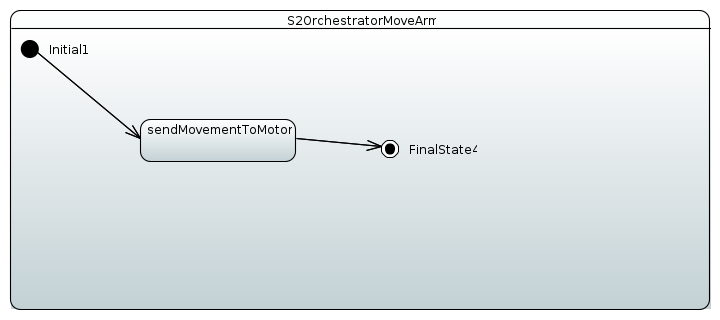
\includegraphics[width=1\linewidth]{pictures/S2OrchestratorMoveArm.PNG}
    \caption{Diagrama de estados del método \texttt{moveArm()} del \textit{orchestrator}.}
    \label{fig:fun_move_arm_orchestator}
\end{figure}

Este método es el encargado de mandar los movimientos a los motores una vez estos se hayan computado.

\begin{itemize}
    \item \texttt{sendMovementToMotors}: se mandan los movimientos necesarios a los motores.
    
\end{itemize}

En el caso del bloque \texttt{UART} tenemos los siguientes diagramas:

\begin{figure}[H]
    \centering
    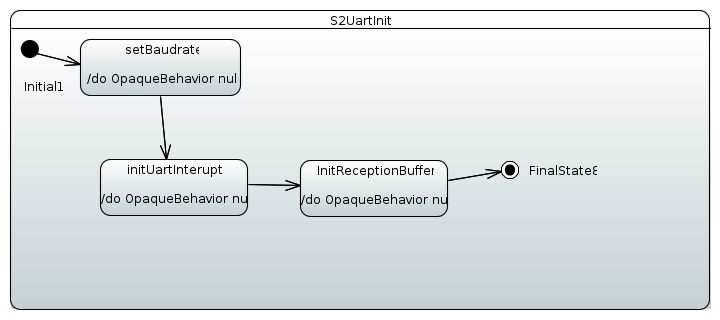
\includegraphics[width=1\linewidth]{pictures/S2UartInit.PNG}
    \caption{Diagrama de estados del método \texttt{uartInit()} del \textit{UART}.}
    \label{fig:fun_uart_init_uart}
\end{figure}

Se ejecuta este método al inicio de la comunicación a través de la \ac{UART} para configurar la transmisión de datos.

\begin{enumerate}
    \item \texttt{setBaudrate}: se establece una tasa de baudios para la transmisión asíncrona
    \item \texttt{initUartInterupt}: se configura el registro de interrupciones de tal manera que la \ac{UART} sea capaz de generar una interrupción en el sistema con el objetivo de poder saber cuándo se ha recibido una nueva trama de bits.
    \item \texttt{initReceptionBuffer}: se inicializa el \textit{buffer} de recepción.
\end{enumerate}

\begin{figure}[H]
    \centering
    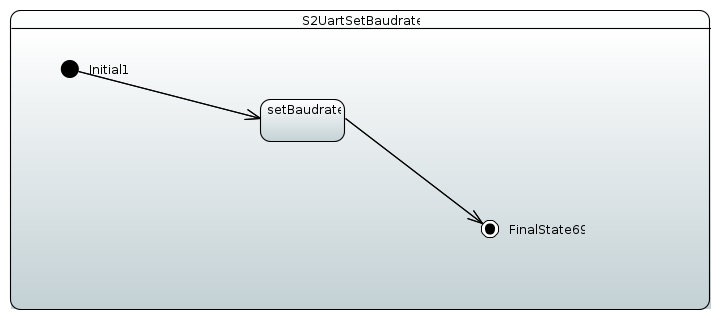
\includegraphics[width=1\linewidth]{pictures/S2UartSetBaudrate.PNG}
    \caption{Diagrama de estados del método \texttt{setBaudrate()} del \textit{UART}.}
    \label{fig:fun_set_baudrate_uart}
\end{figure}

Se configuran los registros necesarios para obtener una tasa de baudios adecuados para la comunicación

\begin{itemize}
    \item \texttt{setBaudrate}: se realiza la configuración que actualiza la tasa de baudios del sistema.
\end{itemize}

\begin{figure}[H]
    \centering
    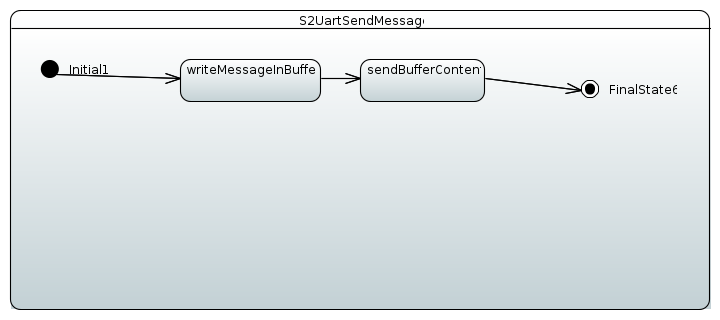
\includegraphics[width=1\linewidth]{pictures/S2UartSendMessage.PNG}
    \caption{Diagrama de estados del método \texttt{sendMessage()} del \textit{UART}.}
    \label{fig:fun_send_message_uart}
\end{figure}

Se escribe un mensaje en el \textit{buffer} de envío y este es posteriormente enviado.

\begin{enumerate}
    \item \texttt{writeMessageInBuffer}: se escribe el mensaje en el \textit{buffer} de salida de la \ac{UART}.
    \item \texttt{sendBufferContent}: se envía el contenido del buffer a \ac{S1}.
\end{enumerate}

\begin{figure}[H]
    \centering
    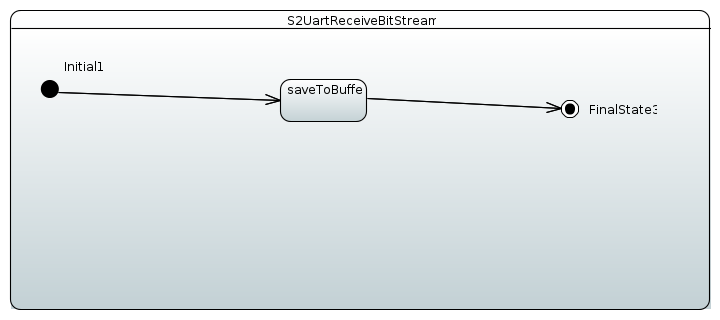
\includegraphics[width=1\linewidth]{pictures/S2UartReceiveBitStream.PNG}
    \caption{Diagrama de estados del método \texttt{receiveBitStream()} del \textit{UART}.}
    \label{fig:fun_receive_bit_stream_uart}
\end{figure}

Se guarda un mensaje en el \textit{buffer} de recepción.

\begin{itemize}
    \item \texttt{saveToBuffer}: se escribe el mensaje en el \textit{buffer} de entrada de la \ac{UART}.
\end{itemize}


En el caso del bloque \texttt{MotorHandler} tenemos los siguientes diagramas:

\begin{figure}[H]
    \centering
    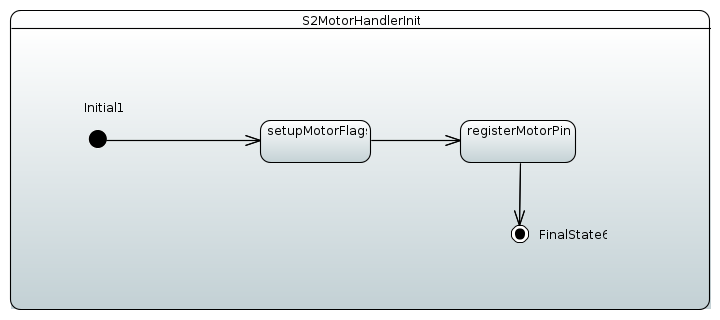
\includegraphics[width=1\linewidth]{pictures/S2MotorHandlerInit.PNG}
    \caption{Diagrama de estados del método \texttt{init()} del \textit{motorHandler}.}
    \label{fig:fun_init_motor_handler}
\end{figure}

Se inicializan los \textit{flags} y se registran los pines a los que están conectados los motores.

\begin{enumerate}
    \item \texttt{setupMotorFlags}: se establecen los flags de los motores.
    \item \texttt{registerMotorPin}: se registran los pines físicos a los que están conectados los motores con el objetivo de saber donde se deben enviar las señales \ac{PWM}.
\end{enumerate}

\begin{figure}[H]
    \centering
    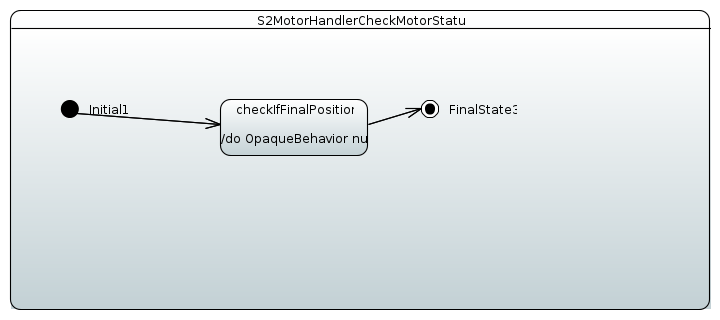
\includegraphics[width=1\linewidth]{pictures/S2MotorHandlerCheckMotorStatus.PNG}
    \caption{Diagrama de estados del método \texttt{checkMotorStatus()} del \textit{motorHandler}.}
    \label{fig:fun_check_motor_status_motor_handler}
\end{figure}

Este método sirve para asegurar que los motores se encuentran en buenas condiciones de funcionamiento.

\begin{itemize}
    \item \texttt{checkIfFinalPosition}: se envía a los motores a una posición en la que se sabe que debería estar en contacto con algún fin de carrera y, posteriormente, se verifica que dichos fines de carrera están activados. De esta manera se asegura que los motores pueden girar.
\end{itemize}

\begin{figure}[H]
    \centering
    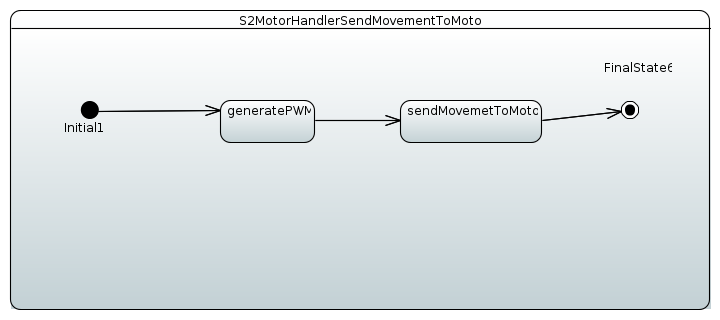
\includegraphics[width=1\linewidth]{pictures/S2MotorHandlerSendMovementToMotors.PNG}
    \caption{Diagrama de estados del método \texttt{sendMovementToMotors()} del \textit{motorHandler}.}
    \label{fig:fun_send_movement_to_motors_motor_handler}
\end{figure}

Se genera una señal PWM y se envía al motor correspondiente

\begin{enumerate}
    \item \texttt{generatePWM}: en base al vector de movimientos que se obtiene a través del \textit{orchestator} y del \textit{movementComputer} se generar las señales PWM necesarias para poder realizarlos.
    
    \item \texttt{sendMovementToMotor}: se envía la seña \ac{PWM} al motor.
\end{enumerate}

\begin{figure}[H]
    \centering
    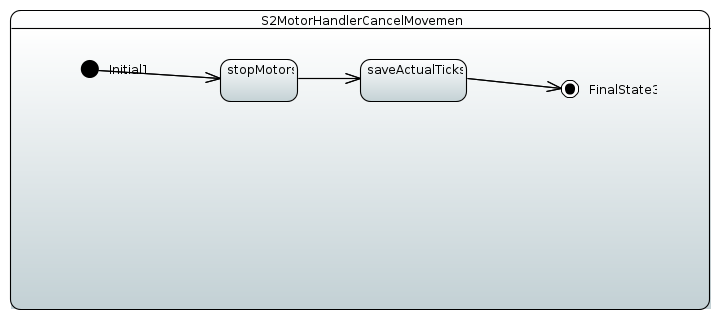
\includegraphics[width=1\linewidth]{pictures/S2MotorHandlerCancelMovement.PNG}
    \caption{Diagrama de estados del método \texttt{cancelMovement()} del \textit{motorHandler}.}
    \label{fig:fun_cancel_movement_motor_handler}
\end{figure}

Se cancela un movimiento que se este ejecutando actualmente.

\begin{enumerate}
    \item \texttt{stopMotor}: se para el motor.
    \item \texttt{saveActualTicks}: se guardan los \textit{ticks} actuales que el motor ha recorrido. Los \textit{ticks} representan ciclos de instrucción durante los cuales el motor recibe una señal \ac{PWM} específica. Se entra en detalle sobre este aspecto en apartados posteriores del documento.
\end{enumerate}

En el caso del bloque \texttt{MovementComputer} tenemos los siguientes diagramas:

\begin{figure}[H]
    \centering
    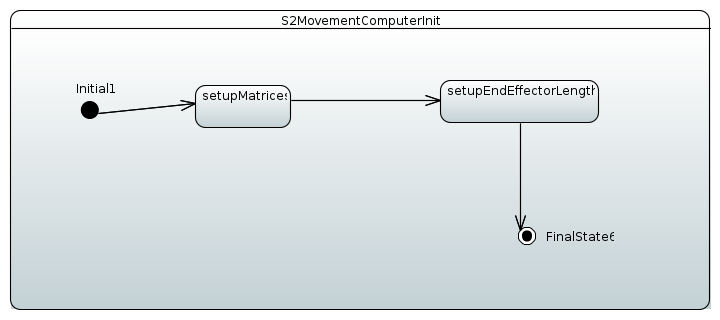
\includegraphics[width=1\linewidth]{pictures/S2MovementComputerInit.PNG}
    \caption{Diagrama de estados del método \texttt{init()} del \textit{movementComputer}.}
    \label{fig:fun_init_movement_computer}
\end{figure}

Se inicializan las matrices de la cinemática directa y se define la distancia del \textit{end--effector} desde la base del brazo.

\begin{enumerate}
    \item \texttt{setupMatrices}: se inicializan las matrices de la cinemática directa.
    \item \texttt{setupEndEffectorLength}: se definen la distancia desde la base hasta el \textit{end--effector}.
\end{enumerate}

\begin{figure}[H]
    \centering
    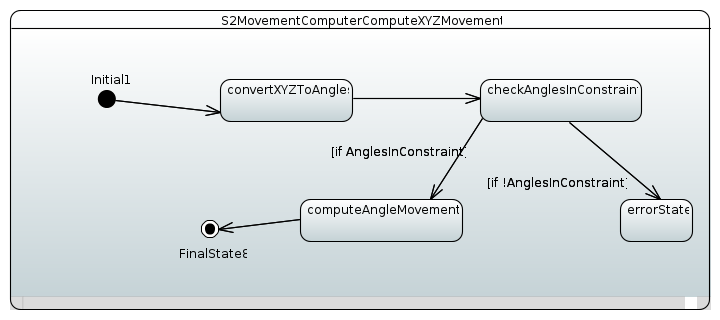
\includegraphics[width=1\linewidth]{pictures/S2MovementComputerComputeXYZMovement.PNG}
    \caption{Diagrama de estados del método \texttt{computeXYZMovement()} del \textit{movementComputer}.}
    \label{fig:fun_compute_xyz_movement_movement_computer}
\end{figure}

\begin{enumerate}
    \item \texttt{convertXYZToAngles}: se emplea la cinemática inversa para obtener la posición de los motores a partir de la posición del \textit{end--effector}
    \item \texttt{checkAnglesInConstraint}: Se verifica si los ángulos están dentro de las limitaciones de los motores.
    \item \texttt{computeAngleMovement}: Se calcula el movimiento que se debe realizar para mover el \textit{end--effector} desde la posicion actual a la deseada.
    \item \texttt{errorState}: Estado de error al que se llega si en alguno de los estados ocurre algún problema inesperado. 
\end{enumerate}

\begin{figure}[H]
    \centering
    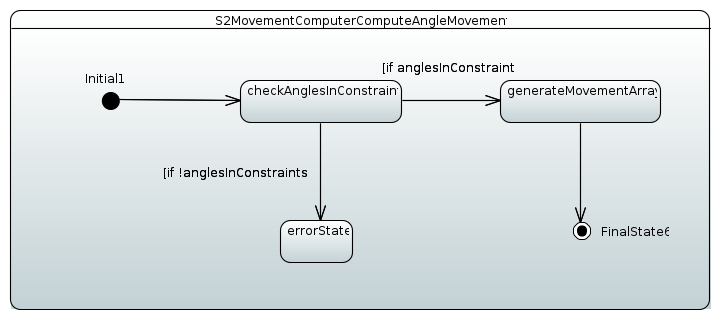
\includegraphics[width=1\linewidth]{pictures/S2MovementComputerComputeAngleMovement.PNG}
    \caption{Diagrama de estados del método \texttt{computeAngleMovement()} del \textit{movementComputer}.}
    \label{fig:fun_compute_angle_mocement_movement_computer}
\end{figure}

\begin{enumerate}
    \item \texttt{checkAnglesInConstraint}: se verifica si los ángulos están dentro de las limitaciones de los motores.
    \item \texttt{generateMovementArray}: se generan los vectores de movimientos.
    \item \texttt{errorState}: estado de error al que se llega si en alguno de los estados ocurre algún problema inesperado. 
\end{enumerate}